\section{Óptica geométrica}
\capequation{Índice de refracción}
\begin{itemize}
    \item Absoluto
    \begin{equation}
        n = \frac{c_o}{v_p}
    \end{equation}
    \item Relativo
    \begin{equation}
        n = \frac{n_1}{n_0}
    \end{equation}
\end{itemize}

\capequation{Ley de Snell}
\begin{equation}
    n_1 \sin{\theta_1} = n_2 \sin{\theta_2}
\end{equation}

\capequation{Corrimiento lateral en láminas de caras paralelas}
\begin{itemize}
    \item h (Espesor de la placa)
    \item d (Desviación)
    \item $\theta_i$ (Ángulo incidente Snell)
    \item $\theta_r (\beta)$ (Ángulo reflejado Snell)
\end{itemize}
\begin{equation}
    d = \frac{\sin{(\theta_i - \theta_r)} \cdot h}{\cos{(\theta_r)}}
\end{equation}
\begin{figure}[h]
    \centering
    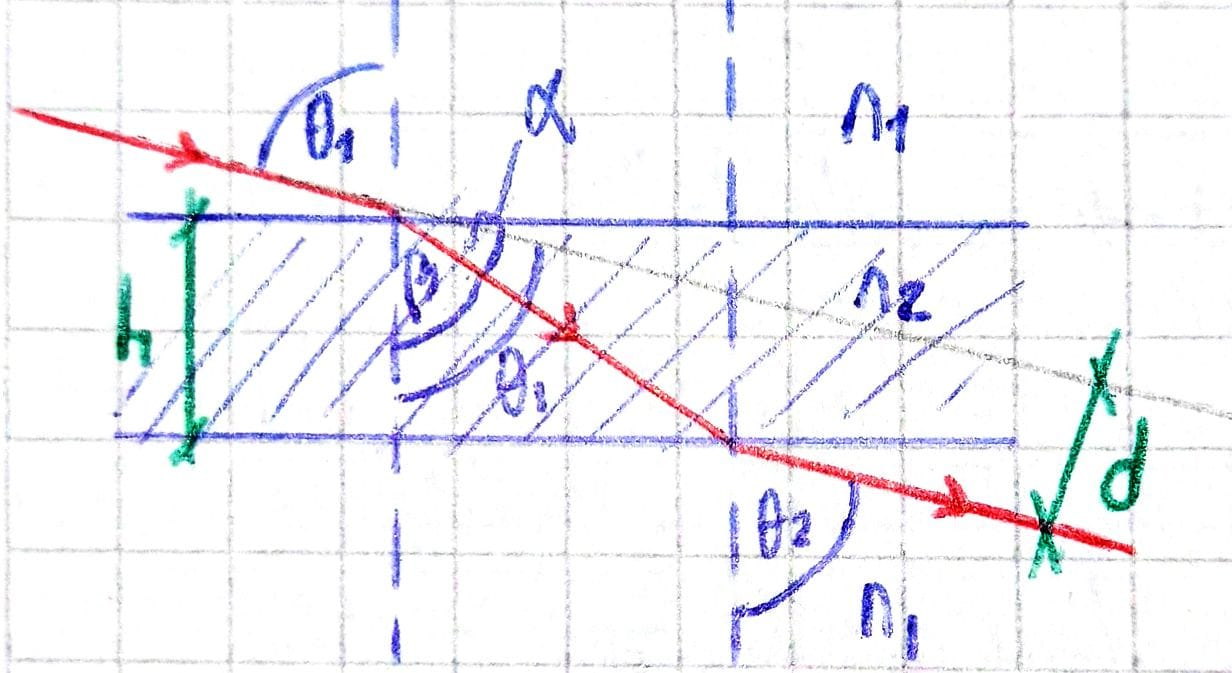
\includegraphics[scale=0.12]{images/laminas_paralelas.png}
\end{figure}

\capequation{Longitud óptica}
\begin{itemize}
    \item n (Índice de refracción)
    \item S (Espesor de la superficie)
\end{itemize}
\begin{equation}
    L_{opt} = n_i \cdot S_i
\end{equation}

\capequation{Fórmula de Descartes para espejos esféricos}
\begin{itemize}
    \item X (Posición del objeto)
    \item X' (Posición de la imagen)
    \item F (Foco del espejo)
    \item R (Radio de curvatura del espejo)
    \begin{equation}
        \frac{1}{X} + \frac{1}{X'} = \frac{1}{F} + \frac{2}{R} 
    \end{equation}
    \item El foco en un es espejo es único y es
    \begin{equation*}
        f = \frac{R}{2}
    \end{equation*}
    \begin{equation*}
        f' = \frac{R}{2}
    \end{equation*}
\end{itemize}

\capequation{Aumentos en espejos}
\begin{equation}
    A = \frac{X'}{X} = -\frac{Y'}{Y}
\end{equation}

\capequation{Dioptras esféricas}
\begin{itemize}
    \item Ecuación general
    \begin{equation}
        \frac{n_2}{X'} - \frac{n_1}{X} = \frac{(n_2 - n_1)}{R}
    \end{equation}
    \item Foco objeto
    \begin{equation}
        f = -\frac{n_1 \cdot R}{n_2 - n_1}
    \end{equation}
    \item Foco imagen
    \begin{equation}
        f = \frac{n_2 \cdot R}{n_2 - n_1}
    \end{equation}
    \item Relación de focos
    \begin{equation}
        \frac{f}{f'} = -\frac{n_1}{n_2}
    \end{equation}
    \item Notar que si la dioptra es plana el $R\rightarrow \infty$ por lo que queda
    \begin{equation*}
        X' = X \cdot \frac{n_2}{n_1}
    \end{equation*}
    \item La dioptra puede ser convergente o divergente
\end{itemize}

\capequation{Aumentos en dioptras}
\begin{itemize}
    \item Planas $A = +1$ (Aumento unitario. Imagen derecha)
    \item Esféricas
    \begin{equation}
        A = \frac{n_1 \cdot X'}{n_2 \cdot X} = \frac{Y'}{Y}
    \end{equation}
\end{itemize}

\capequation{Lentes}
\begin{itemize}
    \item Las lentes pueden ser convergentes o divergentes y a su vez (geométricamente):
    \begin{itemize}
        \item Bi-convexa
        \item Bi-concava
        \item Plano - Convexa
        \item Plano - Concava
        \item Concava - Convexa (meñisco)
    \end{itemize}
    \item Fórmula general
    \begin{itemize}
        \item $n_l$ (Índice de refracción de la lente)
        \item $n_m$ (Índice de refracción del medio)
    \end{itemize}
    \begin{equation}
        \frac{1}{X} - \frac{1}{X'} = \frac{n_m - n_l}{n_l} \cdot \left( \frac{1}{R_2} - \frac{1}{R_1}\right)
    \end{equation}
    \item Foco Objeto
    \begin{equation}
       \frac{1}{F} = \frac{n_m - n_l}{n_l} \cdot \left( \frac{1}{R_2} - \frac{1}{R_1}\right)
    \end{equation}
    \item Foco Imagen
    \begin{equation}
       -\frac{1}{F'} = \frac{n_m - n_l}{n_l} \cdot \left( \frac{1}{R_2} - \frac{1}{R_1}\right)
    \end{equation}
    \item Si los focos son virtuales (divergente), si son reales (convergentes)
\end{itemize}

\capequation{Aumentos en lentes}
\begin{equation}
    A = \frac{X'}{X} = \frac{Y'}{Y}
\end{equation}

\capequation{Potencia de una lente}
\begin{itemize}
    \item Se mide en \textit{dioptrías} $\left[\frac{1}{m}\right]$
    \begin{equation}
        P = \frac{1}{F} = \frac{n_m - n_l}{n_l} \cdot \left( \frac{1}{R_2} - \frac{1}{R_1}\right)
    \end{equation}
\end{itemize}

\capequation{Prismas}
\begin{figure}[h]
    \centering
    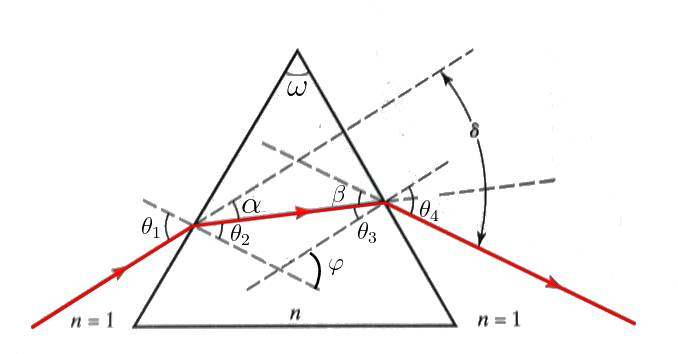
\includegraphics[scale=0.3]{images/prisma.jpg}
\end{figure}
\begin{itemize}
    \item El ángulo A de la imagen lo llamaré $\omega$
    
    \item Para ángulos pequeños la desviación mínima será
    \begin{equation}
        \delta_{min} = (n-1) \omega
    \end{equation}
    \item Para conocer el índice del prisma
    \begin{equation}
        n = \frac{\sin(\frac{\delta_{min} + \omega}{2})}{\sin(\frac{\omega}{2})}
    \end{equation}
    \item Ángulos notables
        \begin{align*}
            \alpha    &= \theta_1 - \theta_2  & \beta  &= \theta_4 - \theta_3 \\
            \theta_2  &= \frac{\omega}{2}     & \delta &= \theta_1 + \theta_4 - \omega \\
        \end{align*}
        ($2\theta_1$ es porque $\theta_1 = \theta_4$)
        \begin{equation*}
            \delta_{min} = 2\theta_1 - \omega
        \end{equation*}
\end{itemize}
\newpage